% -*- TeX-master: "sbml-level-2-version-4"; fill-column: 66 -*-
% $Id$
% $HeadURL$
% ----------------------------------------------------------------

\section{XML Schema for SBML}
\label{apdx:schema}

The following is an XML Schema definition for SBML Level~2 Version~3, using
the W3C Recommendation for XML Schema version~1.0 of 2 May
2001~\citep{biron:2000,fallside:2000,thompson:2000}.  This Schema
does not define all aspects of SBML Level 2: an SBML document
validated by this schema is not necessarily a valid \sbmltwo
document.  Appendix~\ref{apdx:mathml-subset-schema} contains a a
schema for the SBML MathML subset.
Appendix~\ref{apdx:validation-rules} contains a list of the
remaining checks required to validate a model in addition
to making it consistent with these two schemas.

Note to implementors: the following schema is
self-contained and makes reference to the official XML Schema for
MathML hosted at the W3.  However, for use in software systems, it
is more efficient to store the MathML subset Schema of
Appendix~\ref{apdx:mathml-subset-schema} in a file on a user's
local disk, and change the \token{schemaLocation} value on line 27
below to refer to this local copy of the MathML subset Schema.
Doing so will avoid requiring a network access every time this
SBML Schema is used.

\begin{example}
\begin{footnotesize}
\documentclass[10pt]{cek-article}
\usepackage{amsmath}
\usepackage{amssymb}
\usepackage[dvips]{graphicx}
\usepackage{array}
\usepackage{html}
\usepackage[dvips]{color}

\renewcommand{\arraystretch}{1.1}
\pagecolor{white}

% Miscellaneous macros.

\newcommand{\bN}{\mbox{\boldmath $N$}}
\newcommand{\bZero}{\mbox{\boldmath $0$}}
\newcommand{\bLo}{\mbox{\boldmath $L_0$}}
\newcommand{\bNo}{\mbox{\boldmath $N_0$}}
\newcommand{\bNr}{\mbox{\boldmath $N_R$}}
\newcommand{\D}{\displaystyle}

\newcommand{\boxedgraphic}[2][]{\def\fboxsep{0pt}\fbox{\includegraphics[#1]{#2}}}

\newcommand{\notationdocloc}{\url{ftp://ftp.cds.caltech.edu/pub/caltech-erato/notation/}}
\newcommand{\eratowebloc}{\url{http://www.cds.caltech.edu/erato/}}

\begin{document}

%=============================================================================
% Title page
%=============================================================================

\title{An XML-Based Model Description Language\\
    for Systems Biology Simulations}

% The silliness with the begin{latexonly}/begin{htmlonly} is because
% latex2html barfs on the \author command, for reasons that are not clear.
% This was the easiest workaround I could find.  2000-10-17 <mhucka@caltech.edu>

\begin{latexonly}
  \author{Andrew Finney, Herbert Sauro, Michael Hucka, Hamid Bolouri\\[-2 pt]
    \normalsize\texttt{\{afinney,hsauro,mhucka,hbolouri\}@cds.caltech.edu}\\[-4pt]
    \normalsize ERATO Kitano Systems Biology Project\\[-4pt]
    \normalsize Control and Dynamical Systems 107-81\\[-4pt]
    \normalsize California Institute of Technology, Pasadena, CA 91125\\[4pt]
    \normalsize This document is based on discussions with the authors of\\[-4pt]
    \normalsize BioSpice (Arkin), DBSolve (Goryanin), E-Cell (Tomita, Nakayama, Takahashi), Gepasi (Mendez),\\[-4pt]
    \normalsize Jarnac (Sauro), StochSim (Bray, Firth \& Shimizu), Virtual Cell (Loew \& Schaff),\\[-4pt]
    \normalsize and the ERATO Kitano Systems Biology Project group.}
\end{latexonly}

\date{Version of \today{}}

\maketitle

\begin{htmlonly}
\begin{center}
  Andrew Finney, Herbert Sauro, Michael Hucka, Hamid Bolouri\\
  \texttt{\{afinney,hsauro,mhucka,hbolouri\}@cds.caltech.edu}\\
  ERATO Kitano Systems Biology Project\\
  Control and Dynamical Systems 107-81\\
  California Institute of Technology, Pasadena, CA 91125\\
  \\
  This document is based on discussions with the authors of\\
  BioSpice (Arkin), DBSolve (Goryanin), E-Cell (Tomita, Nakayama, Takahashi), Gepasi (Mendez),\\
  Jarnac (Sauro), StochSim (Bray, Firth \& Shimizu), Virtual Cell (Loew \& Schaff),\\
  and the ERATO Kitano Systems Biology Project group.
\end{center}
\end{htmlonly}

% Stick the table of contents on the front page.
% The following settings tweak the format to something nicer than the default.

\setcounter{tocdepth}{2}
\addtolength{\parskip}{-1.2 ex}
\small
\tableofcontents
\normalsize
\addtolength{\parskip}{1.2 ex}            % Undo the effects of previous adj.

\newpage

%=============================================================================
\section{Introduction}
\label{sec:introduction}
%=============================================================================

We present a first attempt at specifying a common, model-based
description language for systems biology simulation software.  We
call this this the \underline{S}ystems \underline{B}iology
\underline{M}arkup \underline{L}anguage (SBML).  The overall goal
is to develop an {\bfseries open standard} that will enable
simulation software to communicate and exchange models,
ultimately leading to the ability for researchers to run
simulations and analyses across multiple software packages.

SBML is the result of merging the most obvious modeling-language features
of BioSpice, DBSolve, E-Cell, Gepasi, Jarnac, StochSim, and Virtual Cell.
The description language is encoded in XML, the Extensible Markup
Language~(Bosak and Bray, 1999; Bray, Paoli and Sperberg-McQueen, 1998).
The XML encoding of the description language can define a file format;
however, at this time, we are focusing on using the XML-based description
language as an interchange format for use in communications between
programs.

The primary purpose of this document is to serve as a basis for discussion
and further development of a more comprehensive language specification. The
final outcome of this process will be an XML Schema which can be used to
communicate model descriptions between simulation packages. Appendix
\ref{apdx:schemas} contains the current version of this schema.  As XML
Schemas are difficult to read and absorb by human readers, we define the
proposed data structures using a succinct graphical notation based on a
subset of UML, the Unified Modeling Language (Eriksson, 1998; Oestereich,
1999).  Our notation is explained in \emph{A Notation for Describing Data
  Representations Intended for XML Encoding}~(Hucka, 2000), available
online at \notationdocloc{}.  For the sake of clarity, we ask readers to
use this notation when contributing to discussions about the specification.
To facilitate discussions, a web/FTP site and a group mailing list have
been set up for the participating groups.  Please see the web site at
\eratowebloc{} for details.

A few assumptions about the form of the language are not
necessarily self-evident.  In particular,
\begin{itemize}

\item We assume that, in order for each simulator program to read and write
  the model description language, the program will require native interface
  code or a stream/file converter.  This interface code will have to
  translate the simulator's internal data structures to and from the model
  description language, as well as smooth any out small differences in
  conceptual organization between the simulator's specific internal
  representation and the model description language.

\item A zero value is not the same as an empty attribute value.  The model
  description language uses a number of structures that, in a given object
  instance, may be empty, depending on whether a given simulator needs
  them.  Programs that interpret objects expressed in the language must be
  designed to pay attention to this distinction.

\end{itemize}

The XML definition of SBML follows a certain naming convention~(Hucka,
2000): the names of object attributes begin with a lowercase letter and the
names of object classes or types begin with an uppercase letter.  In this
document, we also follow the convention of writing keywords (names of
types, attributes, elements, etc.) in a typewriter-style font; for example,
\class{Compartment} is a class name and \class{compartment} is an element
name.

Appendix \ref{sec:xml-rep} contains several examples of models encoded in
XML using SBML.  We use portions of these models as illustrations
throughout the rest of this document.


%=============================================================================
\section{Overview}
\label{sec:overview}
%=============================================================================

The representation language is organized around five categories of
information: model, compartment, geometry, specie and reaction.  Not all of
these will be needed by every simulation package; rather, the intent is to
cover the range of data structures needed by the collection of all of the
simulators examined so far.

\begin{figure}
  \centering
  \includegraphics[scale = 0.75]{top-level.eps}
  \caption{A diagram of the highest level of the object class hierarchy.
    (The notation used in the figures in this document is summarized in
    Appendix \ref{appendix:notation}).}
  \label{fig:top-level}
\end{figure}

Figure~\ref{fig:top-level} depicts the highest level of organization of the
objects in SBML.  It shows that all classes are derived either directly or
indirectly from the class \class{Identified}.  \class{Identified} contains
attributes \attrib{id} and \attrib{simpleNotes} and elements \attrib{notes}
and \class{annotation}.  The attribute \attrib{id} has type \class{ID}, so
that \class{Identified} objects can be referred to using the XML
\class{ID}/\class{IDREF} mechanism~(Biron and Malhotra, 2000).  The element
\class{notes} can contain XHTML content.  The \attrib{simpleNotes} is of
type \class{string}.  Both \attrib{notes} and \attrib{simpleNotes} are
intended to store information meant to be presented to humans.  Finally,
the element \attrib{annotation} can contain arbitrary elements and is
intended to store information not necessarily intended for human viewing.
All SBML classes are derived from \class{Identified}.

In SBML, several classes have attributes of the type \class{Name}.  The
\class{Name} type is a XML simple type derived from the XML \class{string}
type, and is defined to have following pattern (expressed here in
conventional Backus-Naur Form [BNF]):
\begin{quote}
\begin{verbatim}
Letter ::= 'a'..'z','A'..'Z'
Digit ::= '0'..'9'
Name ::= Letter | '_' { Letter | '_' | Digit}
\end{verbatim}
\end{quote}

In the following diagrams, we follow the UML convention of omitting the
display of the attributes on subclasses derived from \class{Identified},
although it should be understood that these attributes are always
available.


%=============================================================================
\section{Elements of the Systems Biology Markup Language (SBML)}
\label{sec:elements}
%=============================================================================

In the sections that follow, we discuss each of the major classes
that are derived from \class{Identified} in the representational
hierarchy.


%-----------------------------------------------------------------------------
\subsection{Model}
%-----------------------------------------------------------------------------

The \class{Model} class defines a grouping of components; that is, a model
does not necessarily represent a single specific biological entity.  There
is only one element of type \class{Model} per instance of an SBML document
or data stream, and it contains the list of compartments, species and
reactions that define a given model.  The UML-based definition of the class
is shown in Figure~\ref{fig:model}.

\begin{figure}[htb]
  \centering
  \includegraphics[scale = 0.75]{model.eps}
  \caption{A diagram of \class{Model}.}
  \label{fig:model}
\end{figure}

\newpage

The definition shows that there must be at least one specie, one reaction
and one compartment in a model; otherwise, there would be little point in
defining the model in the first place.  There is no restriction on the
total number of these elements; Appendix~\ref{sub:minimal-eg} gives an
example of a minimal model.  In addition, a model can consist of zero or
more \class{Geometry}, \class{Mapping}, \class{Parameter} and \class{Rule}
elements.  \class{Model} has an optional \attrib{name} attribute of type \class{Name}.

The following is a skeletal example:
\begin{quote}
\begin{small}
\tightspacing
\begin{verbatim}
<sbml version="1">
    <model>
        <listOfCompartments>
        </listOfCompartments>

        <listOfSpecies>
        </listOfSpecies>

        <listOfReactions>
        </listOfReactions>
    </model>
</sbml>
\end{verbatim}
\regularspacing
\end{small}
\end{quote}

%--------------------------------------------------------------------------
\subsubsection{Units}
%---------------------------------------------------------------------------

\class{Model} and other classes have attributes for defining the units
used.  An example that uses this feature is given in
Appendix~\ref{subsection:unitseg}.

SMBL has several predefined quantity types: time, amount of substance,
volume, charge and length.  Apart from amount of substance and charge, these are all
restricted to metric units.  In all cases, apart from charge, the scale of the given value can
be modified using a power-of-ten multiplier which is an optional integer
attribute.  Amount of substance can be expressed in number of molecules,
depending on the state of the \attrib{substanceIsNumberOfMolecules} boolean
attribute.  Table~\ref{tab:builtin} lists the built-in quantity types and
their associated scale attributes.

\begin{table}[tb]
\begin{tabular}{lllll}
                &                         &                      & \textbf{Default} & \\
  \textbf{Type} & \textbf{Attribute Name} & \textbf{Metric Unit} & \textbf{Scale} & \textbf{Applicable Elements} \\
  \hline
  substance & \attrib{substanceScale} & Moles or no. of molecules & 1 & \class{Model}, \class{Specie}, \class{KineticLaw} \\
  time      & \attrib{timeScale}      & Seconds & 1 & \class{Model}, \class{KineticLaw} \\
  volume    & \attrib{volumeScale}    & litres & 1 & \class{Model} \\
  length    & \attrib{lengthScale}    & metres & $10^{-6}$ $(\mu)$ & \class{Model}, \class{Geometry} \\
  charge    &                         & no. of electrons & 1 & \\
\end{tabular}
\caption{A table of the built-in quantities in SBML.}
\label{tab:builtin}
\end{table}

All the scale attributes on \class{KineticLaw}, \class{Specie} and
\class{Geometry} override those on \class{Model}. In various sections
below, these units are combined to define the units involved in formulae.

%This definition shows that \class{Model} in this framework
%is a hierarchical grouping construct.  It does not have geometry or other
%characteristics itself; instead, the \class{Compartment} objects are the
%ones that hold geometries and other attributes.  Compartment objects are
%intented to be the leaf elements in a hierarchical tree, as shown in the
%following illustration, in which the top-most \class{Model}
%object contains two \class{Compartment} objects and another
%\class{Model} object:

%\begin{center}
%  \includegraphics{structure-tree.eps}
%\end{center}

%-----------------------------------------------------------------------------
\subsection{Compartments}
%-----------------------------------------------------------------------------

A \class{Compartment} represents a bounded container in which species are
located.  A diagram of the definition of \class{Compartment} is shown in
Figure~\ref{fig:compartment}.  A \class{Compartment} object has a
\attrib{name} attribute of type \class{Name}.

\begin{figure}[htb]
  \centering
  \includegraphics[scale = 0.75]{compartment.eps}
  \caption{The \class{Compartment} object class definition.}
  \label{fig:compartment}
\end{figure}

\newpage

The geometric characteristics of a compartment are described using a
\class{Geometry} element and a \class{Mapping} element.  The geometry
information is effectively optional, because a \class{Mapping} element
linking a \class{Compartment} element and a \class{Geometry} element may be
absent.  In such cases, the compartment simply serves as a topological
structure.

For convenience, a compartment has the floating-point attribute
\attrib{volume}, representing the total volume of the compartment in the
units of volume defined on the \class{Model}.  This enables concentrations
of species to be calculated in the absence of geometry specifications.  Any
\class{Geometry} element associated with the compartment then overrides
this value.  The \attrib{volume} attribute is optional and defaults to a
value of 1.

The following is an example of a \class{Compartment} element:
\begin{quote}
\begin{small}
\tightspacing
\begin{verbatim}
<compartment name="cell" volume="1"/>
\end{verbatim}
\regularspacing
\end{small}
\end{quote}

Lists of compartments are itemized within the element
\attrib{listOfCompartments} in a \class{Model} object, as in the
following example:

\begin{quote}
\begin{small}
\tightspacing
\begin{verbatim}
<listOfCompartments>
  <compartment name="cytosol" volume="1"/>
  <compartment name="mitochondria" volume="0.3"/>
</listOfCompartments>
\end{verbatim}
\regularspacing
\end{small}
\end{quote}

%-----------------------------------------------------------------------------
\subsection{Geometry}
%-----------------------------------------------------------------------------

As shown in the definition of \class{Model} in Figure~\ref{fig:model}, a
\class{Model} object can contain zero or more \class{Geometry} elements.
The \class{Geometry} class is intended to provide a means for specifying
morphological characteristics of compartments in simulations.  It is
defined in Figure~\ref{fig:geometry}.  \class{Geometry} has a \attrib{name} attribute of type \class{Name}.

\begin{figure}[thb]
  \centering
  \includegraphics[scale = 0.75]{geometry.eps}
  \caption{The \class{Geometry} object class definition.}
  \label{fig:geometry}
\end{figure}

The dimensionality of a compartment can be one, two or three dimensions,
and a given compartment can have an overall physical size.  These aspects
are determined in an instance of a \class{Geometry} element by which of the
three size attributes are given a value: either \attrib{length} (for 1-D),
\attrib{surfaceArea} (for 2-D), or \attrib{volume} (for 3-D).  Some
examples of different dimensionalities are: DNA stretch (1-D); disks in
photoreceptors (2-D); patch of membrane (2-D); cell nucleus (3-D); and
dendritic spines (3-D).  The size of a compartment may change over the
course of a simulation.  The 2-D geometrical information is a boundary
specification that can take the form of a sequence of connected $(x,y)$
coordinates (\class{Point} elements) in a global reference frame.  (Each
point is connected by a straight line to the next point in the sequence.
The last point in the sequence is connected to the first.  This set of
lines forms the 2D boundary.)

All the values on a \class{Geometry} element and its associated elements
are in length units as defined on the \class{Geometry} element by the
\attrib{lengthScale} attribute.  If these units are not defined on the
\class{Geometry} element, the definition on the enclosing \class{Model} is
used instead.

%-----------------------------------------------------------------------------
\subsection{Mapping}
%-----------------------------------------------------------------------------

A \class{Model} element can contain zero or more \class{Mapping} elements.
A \class{Mapping} element maps a \class{Compartment} element to a
\class{Geometry} element.  Thus, \class{Mapping} has two name attributes,
\attrib{compartment} and \attrib{geometry}.  \class{Mapping} is defined in
Figure~\ref{fig:mapping}.

\begin{figure}[htb]
  \centering
  \includegraphics[scale = 0.75]{mapping.eps}
  \caption{The \class{Mapping} object class definition.}
  \label{fig:mapping}
\end{figure}


%-----------------------------------------------------------------------------
\subsection{Species}
\label{sub:species}
%-----------------------------------------------------------------------------

\emph{Species} comprise all entities that take part in reactions.  The
\class{Specie} class is intended to represent these entities.  These
include simple ions (e.g., protons, calcium), simple molecules (e.g.,
glucose, ATP), and large molecules (e.g., RNA, polysaccharides, and
proteins).  Figure~\ref{fig:specie} presents the definition of
\class{Specie}.  \class{Specie} has a \attrib{name} of type \class{Name}.

\begin{figure}[htb]
  \centering
  \includegraphics[scale = 0.75]{specie.eps}
  \caption{The \class{Specie} object class definition.}
  \label{fig:specie}
\end{figure}

The attribute \attrib{initialAmount}, of type float, is used to set the
initial amount of the specie.  These are in the substance units as defined
on \class{Specie} via the \attrib{substanceScale} and
\attrib{substanceIsNumberOfMolecules} attributes in the way described in
the definition of \class{Model} above.  If these units are not defined on a
\class{Specie} object, the definition on the \class{Model} element is used
instead.

The boolean attribute \attrib{boundaryCondition} determines whether the
amount of the specie is fixed or variable over the course of a simulation.
\attrib{boundaryCondition} is optional and defaults to a value of false.
The attribute \attrib{compartment}, of type \class{Name}, is used to
identify the compartment in which the specie belongs.  The integer
attribute \attrib{charge} indicates the charge on the species (in terms of
electrons, not the SI unit Coulombs).

The following is an example of a minimal \class{specie} element inside a
\class{Model}:
\begin{quote}
  \begin{small}
    \tightspacing
\begin{verbatim}
<specie name="s1" compartment="cell" initialAmount="4"/>
\end{verbatim}
    \regularspacing
  \end{small}
\end{quote}

Lists of species are itemized within \attrib{listOfSpecies} inside a
\class{Model} object, as in the following example:
\begin{quote}
  \begin{small}
    \tightspacing
\begin{verbatim}
<listOfSpecies>
  <specie name="Glucose" compartment="cell" initialAmount="4"/>
  <specie name="Glucose_6_P" compartment="cell" initialAmount="0.75"/>
  ...
</listOfSpecies>
\end{verbatim}
    \regularspacing
  \end{small}
\end{quote}

%-----------------------------------------------------------------------------
\subsection{Parameters}
%-----------------------------------------------------------------------------

A \class{Parameter} element associates a symbol with a float value
so that the symbol can be used in formulae in place of the value.
Figure~\ref{fig:parameter} gives the definition of this class.
\class{Parameter} has a \attrib{name} attribute of type \class{Name}.
\begin{figure}[htb]
  \centering
  \includegraphics[scale = 0.75]{parameter.eps}
  \caption{The \class{Parameter} class definition.}
  \label{fig:parameter}
\end{figure}

The symbol is set by the \attrib{name} attribute and the value is taken
from the \attrib{value} attribute of the \class{Parameter} object.  A
parameter can be associated with either a model or a reaction.  The
parameter elements associated with the model define parameters that are
{\em global} to the whole model; those that are associated with a reaction
{\em overload} the global parameters.  (See
Section~\ref{subsection:namespace} for further details.)

The \class{Parameter} class has an optional integer attribute
called \attrib{scale} which defaults to zero.  As for the
built-in types, the \attrib{scale} attribute is a power of ten
multiplier.

The unit of the parameter \attrib{value} is specified by the set of
optional \class{Unit} elements contained within the \class{parameter}
element.  Each unit element has a \attrib{attribute} of type
\class{UnitKind}.  \class{UnitKind} is an enumeration type consisting of
the following values: ``mole'', ``litre'', ``second'', ``metre'', ``gram'', ``ampere'',
``kelvin'', ``centigrade'', ``candela'', ``radian'', ``streadian'', ``hertz'',
``newton'', ``joule'', ``calorie'', ``watt'', ``coulomb'', ``volt'', ``farad'', ``ohm'',
``weber'', ``tesla'', ``henry'', ``lumen'', ``lux'', ``pascal'', ``siemens'',
``becquerel'', ``gray''.  The attribute \attrib{type} can only have one of the
values listed.  Finally, the \class{Unit} class also has an integer
attribute, \attrib{power}, that represents an exponent modifier to the
\attrib{type} value; its default value is 1.

The following is an example of a simple \class{unit} element:
\begin{quote}
  \begin{small}
    \tightspacing
\begin{verbatim}
<unit type="gram" power="3"/>
\end{verbatim}
    \regularspacing
  \end{small}
\end{quote}

Complex units can be created by placing several \class{unit}
elements inside a \class{Parameter} class object.  The use of
derived units can help reduce the number of elements required.
The following is a more complex example of a single
\class{Parameter} element, showing how a symbol, $Vm$, is defined
to be $3\ mM\ l^{-1}\ s^{-1}$:
\begin{quote}
  \begin{small}
    \tightspacing
\begin{verbatim}
<parameter name="Vm" value="3" scale="-3">
    <unit type="mole"/>
    <unit type="litre" power="-1"/>
    <unit type="second" power="-1"/>
</parameter>
\end{verbatim}
    \regularspacing
  \end{small}
\end{quote}

Lists of parameters are itemized on the \attrib{listOfParameters} element
within a \class{Model}.  For example:
\begin{quote}
\begin{small}
\tightspacing
\begin{verbatim}
<listOfParameters>
  <specie name="Km1" value="2.3"/>
  <specie name="Km2" value="10.7"/>
  ...
</listOfParameters>
\end{verbatim}
\regularspacing
\end{small}
\end{quote}

An example of a full model that uses parameters is presented in
Appendix~\ref{subsection:ruleseg}.


%-----------------------------------------------------------------------------
\subsection{Rules}
%-----------------------------------------------------------------------------

A \class{Model} object can contain a list of \class{Rule} elements.  Figure
\ref{fig:rules} shows the class hierarchy of \class{Rules} classes. The
classes \class{CompartmentRule}, \class{SpeciesRule} and
\class{ParameterRule} are subtypes of the \class{Rule} class. A
\class{Rule} element represents a formula of the form \verb|x = y|.  A
\class{Rule} has a string attribute \attrib{formula} that contains a text
string representing a formula in place of \verb|y|.  \class{Rule} elements
are evaluated in the order given in the XML stream/file, however there is no
restriction on the order.

\begin{figure}[htb]
  \centering
  \includegraphics[scale = 0.75]{rule.eps}
  \caption{The \class{Rule} class definition.}
  \label{fig:rules}
\end{figure}

When the simulation application reads the model specification, it will
build a set of ordinary differential equations (ODE).  These will be used
by the simulator to perform various analyses on the model.  The intent is
that rule expressions are an integral part of the ODE expression list and
must be evaluated by the simulator just before the ODE list.

One of the motivations for including rules like this is to be able to
express the computation of the equilibrium concentrations of fast reactions
and modeling pH.  An example of an XML-encoded model that uses \class{Rule}
elements is given in Appendix~\ref{subsection:unitseg}.

%-----------------------------------------------------------------------------
\subsubsection{CompartmentRule}
%------------------------------------------------------------------------------

The class \class{CompartmentRule} has an attribute, \attrib{compartment},
that has type \class{Name} and is used to store a compartment name.
\class{CompartmentRule} inherits attribute \attrib{formula}, used to store
a formula in volume units that are declared on the referenced compartment
element.  The effect of the rule is to set the referenced compartment
volume to the volume returned by the formula.

%--------------------------------------------------------------------------------
\subsubsection{SpeciesRule}
%---------------------------------------------------------------------------------

The class \class{SpeciesRule} has an attribute, \attrib{species},
that has type \class{Name} and is used to store a species name.
\class{SpeciesRule} inherits the attribute \attrib{formula},
which is used to store a formula in concentration or
$substance/volume$ units. \emph{Substance units} are those that
are declared on the referenced \class{Specie} element, and
\emph{volume units} are those declared on the \class{compartment}
element that contains the \class{Specie}.  The effect of the rule
is to set the referenced species concentration to the
concentration returned by the formula.

%--------------------------------------------------------------------------------
\subsubsection{ParameterRule}
%--------------------------------------------------------------------------------

The class \class{ParameterRule} has attributes \attrib{name},
\attrib{scale} and \attrib{unit}.  The \attrib{name} attribute has type
\class{Name}.  The \attrib{scale} and \attrib{unit} operate in the same way
as in the \class{Parameter} class.  The inherited attribute
\attrib{formula} contains a formula in the units defined by the
\attrib{scale} attribute and \class{unit} elements.  The effect of the rule
is to create a new parameter that can be used in subsequent formulae.  This
parameter has the value returned by the formula in the \attrib{formula}
attribute.

The following is an example of a
\class{listOfRules} element:
\begin{quote}
  \begin{small}
    \tightspacing
\begin{verbatim}
<listOfRules>
    <speciesRule species="s2" formula="k*t/(1+k)"/>
    <parameterRule name="t" formula="h*y"/>
    <compartmentRule compartment="cell" formula="z*t">
</listOfRules>
\end{verbatim}
    \regularspacing
  \end{small}
\end{quote}

%-----------------------------------------------------------------------------
\subsection{Formulae}
%-----------------------------------------------------------------------------

Two classes, \class{KineticLaw}, and \class{Rule} have the string attribute
\attrib{formula} that contains formulae.
The attribute values are interpreted as expressions that evaluate to a
floating-point value.

%--------------------------------------------------------------------
\subsubsection{Operators}
%--------------------------------------------------------------------

All operators in formulae return floating-point values.  For boolean
operators, 0 is interpreted as ``false'' and all other values are
interpreted as ``true''.  The operators available are
shown in Table \ref{tab:operators}.

\begin{table}[b]
\begin{center}
\begin{tabular}{lllll}
 \textbf{Tokens} & \textbf{Operator} & \textbf{Class} & \textbf{Precedence} & \textbf{Associates} \\
\hline
\emph{names} & names & primary & 8 & n/a \\
(\emph{expression}) & sub expression & primary & 8 & n/a\\
\emph{f}(\emph{...}) & function call & prefix & 8 & left\\
not, ! & logical not & unary & 7 & right\\
- & negation & unary & 6 & right\\
\verb|^| & power & binary & 5 & left \\
* & multiplication & binary & 4 & left\\
/ & division & binary & 4 & left\\
+ & addition & binary & 3 & left\\
- & subtraction & binary & 3 & left\\
and, \&\& & logical and & binary & 2 & left\\
or, \verb+||+ & logical or & binary & 1 & left\\
xor & logical exclusive or & binary & 1 & left
\end{tabular}
\end{center}
\caption{A table of the expression operators in SBML.  In the
  \textbf{Class} column, ``primary'' implies the construct is an operand,
  ``prefix'' implies the operation is applied to the following arguments,
  ``unary'' implies there is one argument, and ``binary'' implies there are
  two arguments.  The values in the \textbf{Precedence} column show how the
  order of different types of operation are determined.  For example, the
  expression \texttt{a*b+c} is evaluated as \texttt{(a*b)+c} because
  the \texttt{*} operator has higher precedence.  The \textbf{Associates}
  column shows how the order of similar precedence operations is
  determined; for example, \texttt{a - b + c} is evaluated as \texttt{(a -
    b) + c} because the \texttt{+} and \texttt{-} operators are
  left-associative.}
\label{tab:operators}
\end{table}

Simulators do not have to support the logical operators in the near
future.  The operators are listed here simply to reserve the name tokens
for the given operation.

%--------------------------------------------------------------------
\subsubsection{Functions}
%--------------------------------------------------------------------

The function call operator consists of a function name, followed by an
opening parenthesis token (`('), followed by a sequence of zero or more
arguments separated by commas, followed by a closing parenthesis (`)')
token.  Table~\ref{tab:simplemath} in Appendix~\ref{appendix:simplemath}
lists the basic math functions that are defined in SBML at this time.
Table~\ref{tab:ratelaws} in Appendix~\ref{appendix:ratelaws} lists all the
built-in rate law functions.

%--------------------------------------------------------------------
\subsubsection{Symbols}
%--------------------------------------------------------------------

In formulae, the name tokens (other than function names) are the names of
either parameters, parameter rules, compartments or species.  For the
purposes of this document, we call all of them \emph{symbols}.

When a species name occurs in a formula, it represents the concentration
($substance/volume$) of the specie.  The units of the volume are derived
from the \attrib{volumeScale} attribute value on the \class{Model} element
and the substance units defined for the \class{Specie} (see
Section~\ref{sub:species}).

When a compartment name occurs in a formula, it represents the volume of
the compartment.  Again, the units of this value are derived from the
\attrib{volumeScale} attribute value on the \class{Model} element.


%-----------------------------------------------------------------------------
\subsection{Namespaces}
\label{subsection:namespace}
%-----------------------------------------------------------------------------

The names of elements in SBML are constrained.

An element's name is given by the value of the \attrib{name} attribute on
the element.  By default, the name of an element is unique across all the
elements of their element's class, but independent of all other element
names.  For example, reaction names are unique among all reactions in the
model, but a reaction can have the same name as a compartment.  This rule
establishes a \emph{global namespace} for each class.

Symbols declared outside a reaction element are treated slightly
differently, in that they all have the same namespace.  That is, a
symbol is unique among all other symbols but is independent of
all other element names.

The names of parameter elements contained in a \class{reaction} element are
unique to just the reaction and override symbol names declared elsewhere.
That is, parameter symbols can be defined in one of two names spaces, a
local space confined to particular rate laws, and a global space.  The
advantage of this approach is the following.  Some simulators currently use
a local name space approach when declaring rate laws.  This allows them to
use the same symbol (but different instance) in many different rate laws,
reducing the burden on the modeller when collating a set of parameter
names.  On the other hand, some simulators require the user to generate
unique symbol names for every distinct parameter.  To accomodate this
approach, we introduced the global name space.  In addition, the global
namespace allows sets of rate equations and rules to share the same
parameter symbol (single instance).  For example, a particular enzyme might
catalyze a number of different reactions, in which case it would be an
advantage to specific a single parameter indicating the concentration of
enzyme that would appear in all the effected rate laws.

%-----------------------------------------------------------------------------
\subsection{Reactions}
%-----------------------------------------------------------------------------

A \class{Reaction} represents some transformation, transport or binding
process, typically a chemical reaction, that can change the amount of one
or more species.  \class{Reaction} is defined in Figure~\ref{fig:reaction}.
In this framework, reactions are defined using lists of reactant species,
products, and their stoichiometries, and by parameter values for
separately-defined kinetic laws.  \class{Reaction} has a boolean attribute,
\attrib{reversible}, that has a value of ``false'' by default.

\begin{figure}[htb]
  \centering
  \includegraphics[scale = 0.75]{reaction.eps}
  \caption{The \class{Reaction} object class definition.}
  \label{fig:reaction}
\end{figure}

The examples in Appendix \ref{sec:xml-rep} clarify how the
elements of the \class{Reaction} class are intended to be used.

%-----------------------------------------------------------------------------
\subsubsection{SpeciesReference}
%-----------------------------------------------------------------------------

An instance of \class{SpeciesReference} links a specie to a
\class{Reaction}.  This implies that the reaction will affect the amount of
that specie. The attribute \attrib{specie}, of type \class{Name}, in the
\class{SpecieReference} class in Figure~\ref{fig:reaction} is intended to
refer to the name of a specie in the species list of the \class{Model}.  In
other words, the species involved in a reaction are listed once in a
\class{Model} and the \attrib{listOfReactants} and \attrib{listOfProducts}
in reactions refer to the list of species.  The instances of
\class{SpeciesReference} are \class{specieReference} elements
in the \attrib{listOfReactants} and \attrib{listOfProducts}.

The following is a simple example of a \class{specieReference} element:
\begin{quote}
  \begin{small}
    \tightspacing
\begin{verbatim}
<specieReference specie="X0" stoichiometry="1"/>
\end{verbatim}
    \regularspacing
  \end{small}
\end{quote}

The effective stoichiometry value is created by dividing the
\attrib{stoichiometry} attribute value by the
\attrib{denominator} attribute value. The attribute
\attrib{stoichiometry} is of type integer and is optional,
defaulting to 1. The attribute \attrib{denominator} is of type
integer and is optional, defaulting to 1. (This allows the user to
employ rational arithmetic computations on the stoichiometry
matrix. This helps to eliminate roundoff errors and other
problems during the computation, especially for large matrices.
These computations are particularly important when calculating
things like elementary modes.) Note that the denominator attribute is
{\bfseries optional}.

If the reaction depends on the reactant binding order, such as in
an ordered bi-bi reaction, then the order in which the substrate
and products bind and leave the enzyme is given by the order of
the reactants and products in their respective lists.

%-----------------------------------------------------------------------------
\subsubsection{KineticLaw}
%-----------------------------------------------------------------------------

A \class{kineticLaw} element describes the rate of the enclosing reaction.
The \attrib{formula}, of type \class{string}, expresses the rate in
$substance/time$ units. The exact units for substance and time used can be
given via the \attrib{substanceScale}, \attrib{timeScale} and
\attrib{substanceIsNumberOfMolecules} attributes on \class{KineticLaw} in
the same way described in the \class{Model} section above.  These
attributes are optional and the default values are taken from the
\class{Model} element.

The \class{KineticLaw} element contained in a \class{Reaction} element is
optional; however, in general there is no default element that can be
substituted in place of a missing \class{kineticLaw} element.
\class{KineticLaw} contains zero or more \class{parameter} elements that
define symbols that can be used in the formula string.  These symbols
overload those defined at the \class{Model} level.

The following is a simple example of a \class{KineticLaw} element.
\begin{quote}
  \begin{small}
    \tightspacing
\begin{verbatim}
<kineticLaw formula="k1*X0">
    <listOfParameters>
        <parameter name="k1" value="0"/>
    </listOfParameters>
</kineticLaw>
\end{verbatim}
    \regularspacing
  \end{small}
\end{quote}

%-----------------------------------------------------------------------------
\subsubsection{An Example of a Complete Reaction Element}
%------------------------------------------------------------------------------

The following is an example of a \class{reaction} element and
defines the reaction

\begin{tabular}{@{}lr@{}}
\begin{minipage}[t]{2in}
$$ J_1: \ X_o \longrightarrow S_1; \ k_1 X_0 $$
\end{minipage}
&
\begin{minipage}[t]{3in}
\begin{quote}
  \begin{small}
    \tightspacing
\begin{verbatim}
<reaction name="J1">
    <listOfReactants>
        <specieReference specie="X0" stoichiometry="1"/>
    </listOfReactants>
    <listOfProducts>
        <specieReference specie="S1" stoichiometry="1"/>
    </listOfProducts>
    <kineticLaw formula="k1*X0">
        <listOfParameters>
            <parameter name="k1" value="0"/>
        </listOfParameters>
    </kineticLaw>
</reaction>
\end{verbatim}
    \regularspacing
  \end{small}
\end{quote}
\end{minipage}
\end{tabular}

%------------------------------------------------------------------------------
\section{Versions of the Markup Language}
%------------------------------------------------------------------------------

The top level element \class{sbml} has the integer attribute
\attrib{version} which indicates the version number of the SBML
definition with which the XML stream/file complies.


%------------------------------------------
\section{Future Enhancements}
%-------------------------------------------

We are currently considering the following features for future versions of
SBML:

\begin{itemize}

\item \emph{Literature References}.  This feature will allow the models to
  be annotated with references to papers and authors.

\item \emph{Explicit references to ODEs}.  A model should be able to
  explicitly specify ordinary differential equations alongside the rules
  and reactions. One application of this would be to allow the modelling of
  variable volume spaces.

\item \emph{Submodels}.  This feature will allow the reuse of model
  libraries and the creation of several instances of the same model.

\item \emph{Indices}.  This feature will allow sets of similar reactions to
  be defined that transform sets of species.  A Formula string could then
  include `sum' and `product' functions.

\item \emph{DNA}.  This feature will allow DNA to be explicitly modeled.

\item \emph{Diagrams}.  This feature will allow elements to be annotated
  with data to enable the display of the model in a diagram.

\item \emph{Multiple state species}. This feature will allow species to have multiple states.

\end{itemize}

%=============================================================================
\section{Your Comments}
\label{sec:what}
%=============================================================================

Please use the group email address (\texttt{sysbio@caltech.edu})
and web site \eratowebloc{} to send us your comments and
suggestions.


\setcounter{secnumdepth}{-1}
\section{Appendix}
\setcounter{secnumdepth}{2}

\appendix

%=============================================================================
\section{Using the XML Encoding of SBML}
\label{sec:xml-rep}
%=============================================================================

In this section, we present an example of translating a model into the
systems biology model description language defined in this document.  Our
approach to translating the object class definitions presented in the
sections above is described in the companion document, \emph{A Notation for
  Describing Model Representation Intended for XML Encoding}~(Hucka, 2000).
Appendix~\ref{apdx:schemas} gives the full listing of a preliminary version
of an XML Schema corresponding to SBML, the Systems Biology Markup Language.

%-----------------------------------------------------------------------------
\subsection{Minimal Model}
\label{sub:minimal-eg}
%-----------------------------------------------------------------------------

The following is an example of a model that uses the minimum number of
elements and attributes possible in SBML.
\begin{quote}
  \begin{small}
    \tightspacing
\begin{verbatim}
<sbml version="1">
    <model>
        <listOfCompartments>
            <compartment name="x"/>
        </listOfCompartments>
        <listOfSpecies>
            <specie name="y" compartment="x" initialAmount="1"/>
        </listOfSpecies>
        <listOfReactions>
            <reaction name="x">
                <listOfReactants>
                    <specieReference specie="y"/>
                </listOfReactants>
                <listOfProducts>
                    <specieReference specie="y"/>
                </listOfProducts>
            </reaction>
        </listOfReactions>
    </model>
</sbml>

\end{verbatim}
    \regularspacing
  \end{small}
\end{quote}

%-----------------------------------------------------------------------------
\subsection{A Simple Example Application of SBML}
%-----------------------------------------------------------------------------

The following example is the main portion of an XML document that
describes a simple branch system of the following form:
\[
\begin{array}{ccc}
  & {k1 * X0}\\
  X0 & \longrightarrow & S1
\end{array}
\]
\[
\begin{array}{ccc}
  & {k2 * S1}\\
  S1 & \longrightarrow & X1
\end{array}
\]
\[
\begin{array}{ccc}
  & {k3 * S1}\\
  S1 & \longrightarrow & X2
\end{array}
\]

The following is the XML encoding of the above reaction.
\begin{quote}
\begin{small}
\tightspacing
\begin{verbatim}
<sbml version="1">
    <model id="simplemodel" name="Branch">
        <notes>
            <body xmlns="http://www.w3.org/1999/xhtml">
                <p>Simple branch system.</p>
                <p>The reaction looks like this:</p>
                <p>reaction-1:   X0 -> S1; k1*X0;</p>
                <p>reaction-2:   S1 -> X1; k2*S1;</p>
                <p>reaction-3:   S1 -> X2; k3*S1;</p>
            </body>
        </notes>
        <listOfCompartments>
            <compartment name="compartmentOne" volume="1"/>
        </listOfCompartments>
        <listOfSpecies>
            <specie name="S1" initialAmount="0" compartment="compartmentOne"
                    boundaryCondition="false"/>
            <specie name="X0" initialAmount="0" compartment="compartmentOne"
                    boundaryCondition="true"/>
            <specie name="X1" initialAmount="0" compartment="compartmentOne"
                    boundaryCondition="true"/>
            <specie name="X2" initialAmount="0" compartment="compartmentOne"
                    boundaryCondition="true"/>
        </listOfSpecies>
        <listOfReactions>
            <reaction name="reaction_1" reversible="false">
                <listOfReactants>
                    <specieReference specie="X0" stoichiometry="1"/>
                </listOfReactants>
                <listOfProducts>
                    <specieReference specie="S1" stoichiometry="1"/>
                </listOfProducts>
                <kineticLaw formula="k1*X0">
                    <listOfParameters>
                        <parameter name="k1" value="0"/>
                    </listOfParameters>
                </kineticLaw>
            </reaction>
            <reaction name="reaction_2" reversible="false">
                <listOfReactants>
                    <specieReference specie="S1" stoichiometry="1"/>
                </listOfReactants>
                <listOfProducts>
                    <specieReference specie="X1" stoichiometry="1"/>
                </listOfProducts>
                <kineticLaw formula="k2*S1">
                    <listOfParameters>
                        <parameter name="k2" value="0"/>
                    </listOfParameters>
                </kineticLaw>
            </reaction>
            <reaction name="reaction_3" reversible="false">
                <listOfReactants>
                    <specieReference specie="S1" stoichiometry="1"/>
                </listOfReactants>
                <listOfProducts>
                    <specieReference specie="X2" stoichiometry="1"/>
                </listOfProducts>
                <kineticLaw formula="k3*S1">
                    <listOfParameters>
                        <parameter name="k3" value="0"/>
                    </listOfParameters>
                </kineticLaw>
            </reaction>
        </listOfReactions>
    </model>
</sbml>

\end{verbatim}
  \regularspacing
\end{small}
\end{quote}

The corresponding XML encoding shown above is quite straightforward. The
outermost container is a tag, \texttt{smbl}, that identifies the contents
as being \underline{s}ystems \underline{b}iology \underline{m}arkup
\underline{l}anguage, an application of XML. The next-inner container is a
single \texttt{model} element that serves as the highest-level object in
the model.  The model in this case contains a single \texttt{compartment}
element.

The compartment has four species associated with it, and three reactions.
The correspondence between these elements and the three reaction equations
in the list above should be fairly obvious.  The elements in the
\texttt{listOfReactants} and \texttt{listOfProducts} refer to the names of
elements listed in the \texttt{listOfSpecies}.

The lone \texttt{compartment} has no value for \texttt{volume} because the
value is irrelevant for this particular simple case example.  Since it is
an optional attribute, there is no mention of it in the XML object.

Note that the \texttt{notes} \texttt{annotation} elements of the specie and
reaction elements above have been omitted because they are empty.  The XML
Schema definition in Appendix~\ref{apdx:schemas} is defined in such a way
that these elements are optional.

%-----------------------------------------------------------------------------
\subsection{Simple Use of Units Feature in a Model}
\label{subsection:unitseg}
%-----------------------------------------------------------------------------

The following model uses the units features of SBML.  In this
model, the \attrib{substanceScale} attribute on the \class{model}
element has the value -3 that defines all qualities of substance
to be defined in $10^{-3}$ mole units or milliMoles.  This sets
the default units in the model; elements can override this scale
locally.  The \attrib{volumeScale} and \attrib{timeScale}
attributes are not set, ensuring that volume is in litres and time
is in seconds.  Thus, by default in this model, kinetic law
formulae define rates in milliMoles per second and the specie
symbols in them represent concentration values in milliMoles per
litre.  All the \class{specie} elements set the initial amount of
the given specie to 1 milliMole.

The parameters \texttt{Vm} and \texttt{Km} are defined to be in milliMoles
per Litre per Second and milliMolar respectively.

\begin{quote}
\begin{small}
\tightspacing
\begin{verbatim}
<sbml version="1">
    <model substanceScale="-3">
        <listOfCompartments>
            <compartment name="cell"/>
        </listOfCompartments>
        <listOfSpecies>
            <specie name="x0" compartment="cell" initialAmount="1"/>
            <specie name="x1" compartment="cell" initialAmount="1"/>
            <specie name="s1" compartment="cell" initialAmount="1"/>
            <specie name="s2" compartment="cell" initialAmount="1"/>
        </listOfSpecies>
        <listOfParameters>
            <parameter name="vm" value="2" scale="-3">
                <listOfUnits>
                    <unit type="mole"/>
                    <unit type="litre" power="-1"/>
                    <unit type="second" power="-1"/>
                </listOfUnits>
            </parameter>
            <parameter name="km" value="2" scale="-3">
                <listOfUnits>
                    <unit type="mole"/>
                </listOfUnits>
            </parameter>
        </listOfParameters>
        <listOfReactions>
            <reaction name="v1">
                <listOfReactants>
                    <specieReference specie="x0"/>
                </listOfReactants>
                <listOfProducts>
                    <specieReference specie="s1"/>
                </listOfProducts>
                <kineticLaw formula="(vm*s1)/(km+s1)"/>
            </reaction>
            <reaction name="v2">
                <listOfReactants>
                    <specieReference specie="s1"/>
                </listOfReactants>
                <listOfProducts>
                    <specieReference specie="s2"/>
                </listOfProducts>
                <kineticLaw formula="(vm*s2)/(km+s2)"/>
            </reaction>
            <reaction name="v3">
                <listOfReactants>
                    <specieReference specie="s2"/>
                </listOfReactants>
                <listOfProducts>
                    <specieReference specie="x1"/>
                </listOfProducts>
                <kineticLaw formula="(vm*s1)/(km+s1)"/>
            </reaction>
        </listOfReactions>
    </model>
</sbml>
\end{verbatim}
  \regularspacing
\end{small}
\end{quote}

%-----------------------------------------------------------------------------
\subsection{A Simple Example Application Using Rules}
\label{subsection:ruleseg}
%-----------------------------------------------------------------------------

The following model represents the pathway $X_0 \rightarrow S_1 \rightarrow
S_2 \rightarrow X_1$, where $S_1 \rightarrow S_2$ is a fast reaction.  The
reaction $S_1 \rightarrow S_2$ is not modeled explicitly; instead, the
effect of the reaction is encapsulated in rules.
\begin{quote}
\begin{small}
\tightspacing
\begin{verbatim}
<sbml version="1">
    <model>
        <listOfCompartments>
            <compartment name="cell" volume="1"/>
        </listOfCompartments>
        <listOfSpecies>
            <specie name="s1" compartment="cell" initialAmount="4"/>
            <specie name="s2" compartment="cell" initialAmount="2"/>
            <specie name="x0" compartment="cell" initialAmount="1"/>
            <specie name="x1" compartment="cell" initialAmount="0"/>
        </listOfSpecies>
        <listOfParameters>
            <parameter name="k1" value="1.2"/>
            <parameter name="k2" value="1000"/>
            <parameter name="k3" value="3000"/>
            <parameter name="k4" value="4.5"/>
        </listOfParameters>
        <listOfRules>
            <parameterRule formula="s1 + s2" name="t"/>
            <parameterRule formula="k3/k2" name="k" />
            <specieRule formula="k*t/(1+k)" species="s2"/>
            <specieRule formula="t-s2" species="s1"/>
        </listOfRules>
        <listOfReactions>
            <reaction name="j1">
                <listOfReactants>
                    <specieReference specie="x0"/>
                </listOfReactants>
                <listOfProducts>
                    <specieReference specie="s1"/>
                </listOfProducts>
                <kineticLaw formula="k1*x0"/>
            </reaction>
            <reaction name="j3">
                <listOfReactants>
                    <specieReference specie="s2"/>
                </listOfReactants>
                <listOfProducts>
                    <specieReference specie="x1"/>
                </listOfProducts>
                <kineticLaw formula="k4*s2"/>
            </reaction>
        </listOfReactions>
    </model>
</sbml>


\end{verbatim}
  \regularspacing
\end{small}
\end{quote}

%=============================================================================
\section{XML Schema for SBML}
\label{apdx:schemas}
%=============================================================================

The following is a first draft of an XML Schema definition for the Systems
Biology Markup Language.  Example applications of this XML Schema are
presented in Appendix~\ref{sec:xml-rep}.

The schema below is well-formed and compiles with the XML Schema standard.
However, the use of \texttt{unique} and \texttt{keyref} elements in this
schema has not been fully validated.  The other elements have been fully
validated.  In practice, the \texttt{unique} and \texttt{keyref} elements
may either need to be commented out or will be ignored, because they are
not supported by most XML parsers.

\begin{small}
\tightspacing
\begin{verbatim}
<?xml version="1.0" encoding="UTF-8"?>
<!DOCTYPE xsd:schema PUBLIC "-//W3C//DTD XMLSCHEMA 19991216//EN" "" [
    <!ENTITY % p 'xsd:'>
    <!ENTITY % s ':xsd'>]>
<xsd:schema xmlns:xsd="http://www.w3.org/1999/XMLSchema">
    <xsd:annotation>
        <xsd:documentation>
          File name   : sbml.xsd
          Description : XML Schema for the Systems Biology Markup Language
          Organization: Caltech ERATO Kitano
          Version     : 1
          Modified    : 2000-09-12 10:58 PDT
        </xsd:documentation>
    </xsd:annotation>
    <!-- Name -->
    <xsd:simpleType base="xsd:string" name="Name">
        <xsd:pattern value="(_|[a-z]|[A-Z])(_|[a-z]|[A-Z]|[0-9])*"/>
    </xsd:simpleType>
    <!-- Identifed -->
    <xsd:complexType name="Identified" abstract="true">
        <xsd:element name="notes" maxOccurs="1" minOccurs="0">
            <xsd:complexType>
                <xsd:any namespace="http://www.w3.org/1999/xhtml"
                         maxOccurs="unbounded" minOccurs="1" processContents="skip"/>
            </xsd:complexType>
        </xsd:element>
        <xsd:element name="annotation" maxOccurs="1" minOccurs="0">
            <xsd:complexType>
                <xsd:any maxOccurs="*" minOccurs="1" processContents="skip"/>
            </xsd:complexType>
        </xsd:element>
        <xsd:attribute name="id" type="xsd:ID" use="optional"/>
        <xsd:attribute name="simpleNotes" type="xsd:string" use="optional"/>
    </xsd:complexType>
    <!-- listOfParameters -->
    <xsd:element name="listOfParameters">
        <xsd:complexType>
            <xsd:element name="parameter" type="Parameter" minOccurs="1" maxOccurs="unbounded"/>
        </xsd:complexType>
    </xsd:element>
    <!--listOfUnits-->
    <xsd:element name="listOfUnits">
        <xsd:complexType>
            <xsd:element name="unit" type="Unit" minOccurs="1" maxOccurs="unbounded"/>
        </xsd:complexType>
    </xsd:element>
    <!-- specieReference -->
    <xsd:element name="specieReference" type="SpecieReference"
                 minOccurs="1" maxOccurs="unbounded"/>
    <!-- Model -->
    <xsd:complexType name="Model" base="Identified" derivedBy="extension">
        <xsd:element name="listOfCompartments" minOccurs="1" maxOccurs="1">
            <xsd:complexType>
                    <xsd:element name="compartment" type="Compartment"
                                 minOccurs="1" maxOccurs="unbounded"/>
            </xsd:complexType>
        </xsd:element>
        <xsd:element name="listOfGeometries" minOccurs="0" maxOccurs="1">
            <xsd:complexType>
                    <xsd:element name="geometry" type="Geometry"
                                 minOccurs="1" maxOccurs="unbounded"/>
            </xsd:complexType>
        </xsd:element>
        <xsd:element name="listOfMappings" minOccurs="0" maxOccurs="1">
            <xsd:complexType>
                    <xsd:element name="mapping" type="Mapping"
                                 minOccurs="1" maxOccurs="unbounded"/>
            </xsd:complexType>
        </xsd:element>
        <xsd:element name="listOfSpecies" minOccurs="1" maxOccurs="1">
            <xsd:complexType>
                    <xsd:element name="specie" type="Specie"
                                 minOccurs="1" maxOccurs="unbounded"/>
            </xsd:complexType>
        </xsd:element>
        <xsd:element ref="listOfParameters" minOccurs="0" maxOccurs="1"/>
        <xsd:element name="listOfRules" minOccurs="0" maxOccurs="1">
            <xsd:complexType>
                <xsd:choice maxOccurs="unbounded" minOccurs="1">
                    <xsd:element name="compartmentRule" type="CompartmentRule"
                                 minOccurs="0" maxOccurs="1"/>
                    <xsd:element name="specieRule" type="SpecieRule"
                                 minOccurs="0" maxOccurs="1"/>
                    <xsd:element name="parameterRule" type="ParameterRule"
                                 minOccurs="0" maxOccurs="1"/>
                </xsd:choice>
            </xsd:complexType>
        </xsd:element>
        <xsd:element name="listOfReactions" minOccurs="1" maxOccurs="1">
            <xsd:complexType>
                <xsd:element name="reaction" type="Reaction"
                             minOccurs="1" maxOccurs="unbounded">
                    <xsd:unique name="parameters">
                         <xsd:selector>listOfParameters/parameter</xsd:selector>
                         <xsd:field>@name</xsd:field>
                    </xsd:unique>
                </xsd:element>
            </xsd:complexType>
        </xsd:element>
        <xsd:attribute name="name" type="Name" use="optional"/>
        <xsd:attribute name="substanceScale" type="xsd:integer" use="default" value="0"/>
        <xsd:attribute name="timeScale" type="xsd:integer" use="default" value="0"/>
        <xsd:attribute name="volumeScale" type="xsd:integer" use="default" value="0"/>
        <xsd:attribute name="lengthScale" type="xsd:integer" use="default" value="-6"/>
        <xsd:attribute name="substanceIsNumberOfMolecules" type="xsd:boolean"
                       use="default" value="false"/>
    </xsd:complexType>
    <!-- Compartment -->
    <xsd:complexType name="Compartment" base="Identified" derivedBy="extension">
        <xsd:attribute name="name" type="Name" use="required"/>
        <xsd:attribute name="volume" type="xsd:float" use="default" value="1"/>
    </xsd:complexType>
    <!-- Geometry -->
    <xsd:complexType name="Geometry" base="Identified" derivedBy="extension">
        <xsd:element name="listOfPoints" minOccurs="0" maxOccurs="1">
            <xsd:complexType>
                <xsd:element name="point" type="Point" minOccurs="1" maxOccurs="unbounded"/>
            </xsd:complexType>
        </xsd:element>
        <xsd:attribute name="name" type="Name" use="required"/>
        <xsd:attribute name="length" type="xsd:float" use="optional"/>
        <xsd:attribute name="surfaceArea" type="xsd:float" use="optional"/>
        <xsd:attribute name="volume" type="xsd:float" use="optional"/>
        <xsd:attribute name="lengthScale" type="xsd:integer" use="optional"/>
    </xsd:complexType>
    <xsd:complexType name="Point" base="Identified" derivedBy="extension">
        <xsd:attribute name="x" type="xsd:float" use="required"/>
        <xsd:attribute name="y" type="xsd:float" use="required"/>
    </xsd:complexType>
    <!--Mapping-->
    <xsd:complexType name="Mapping" base="Identified" derivedBy="extension">
        <xsd:attribute name="compartment" type="Name" use="required"/>
        <xsd:attribute name="geometry" type="Name" use="required"/>
    </xsd:complexType>
    <!-- Specie -->
    <xsd:complexType name="Specie" base="Identified" derivedBy="extension">
        <xsd:attribute name="name" type="Name" use="required"/>
        <xsd:attribute name="compartment" type="Name" use="required"/>
        <xsd:attribute name="initialAmount" type="xsd:float" use="required"/>
        <xsd:attributeGroup ref="substanceUnits"/>
        <xsd:attribute name="boundaryCondition" type="xsd:boolean" use="default" value="false"/>
        <xsd:attribute name="charge" type="xsd:integer" use="optional"/>
    </xsd:complexType>
    <!-- Parameter -->
    <xsd:complexType name="Parameter" base="Identified" derivedBy="extension">
        <xsd:element ref="listOfUnits" minOccurs="0" maxOccurs="1"/>
        <xsd:attribute name="value" type="xsd:float" use="required"/>
        <xsd:attribute name="scale" type="xsd:integer" use="default" value="0"/>
        <xsd:attribute name="name" type="Name" use="required"/>
    </xsd:complexType>
    <xsd:simpleType base="xsd:string" name="UnitKind">
        <xsd:enumeration value="mole"/>
        <xsd:enumeration value="litre"/>
        <xsd:enumeration value="second"/>
        <xsd:enumeration value="metre"/>
        <xsd:enumeration value="gram"/>
        <xsd:enumeration value="ampere"/>
        <xsd:enumeration value="kelvin"/>
        <xsd:enumeration value="centigrade"/>
        <xsd:enumeration value="candela"/>
        <xsd:enumeration value="radian"/>
        <xsd:enumeration value="streadian"/>
        <xsd:enumeration value="hertz"/>
        <xsd:enumeration value="newton"/>
        <xsd:enumeration value="joule"/>
        <xsd:enumeration value="calorie"/>
        <xsd:enumeration value="watt"/>
        <xsd:enumeration value="coulomb"/>
        <xsd:enumeration value="volt"/>
        <xsd:enumeration value="farad"/>
        <xsd:enumeration value="ohm"/>
        <xsd:enumeration value="weber"/>
        <xsd:enumeration value="tesla"/>
        <xsd:enumeration value="henry"/>
        <xsd:enumeration value="lumen"/>
        <xsd:enumeration value="lux"/>
        <xsd:enumeration value="pascal"/>
        <xsd:enumeration value="siemens"/>
        <xsd:enumeration value="becquerel"/>
        <xsd:enumeration value="gray"/>
    </xsd:simpleType>
    <xsd:complexType name="Unit" base="Identified" derivedBy="extension">
        <xsd:attribute name="type" type="UnitKind" use="required"/>
        <xsd:attribute name="power" type="xsd:integer" use="default" value="1"/>
    </xsd:complexType>
    <!-- Rule -->
    <xsd:complexType name="Rule" base="Identified" derivedBy="extension" abstract="true">
        <xsd:attribute name="formula" type="xsd:string" use="required"/>
    </xsd:complexType>
    <xsd:complexType name="CompartmentRule" base="Rule" derivedBy="extension">
        <xsd:attribute name="compartment" type="Name" use="required"/>
    </xsd:complexType>
    <xsd:complexType name="SpecieRule" base="Rule" derivedBy="extension">
        <xsd:attribute name="species" type="Name" use="required"/>
    </xsd:complexType>
    <xsd:complexType name="ParameterRule" base="Rule" derivedBy="extension">
        <xsd:element ref="listOfUnits" minOccurs="0" maxOccurs="1"/>
        <xsd:attribute name="name" type="Name" use="required"/>
        <xsd:attribute name="scale" type="xsd:integer" use="default" value="0"/>
    </xsd:complexType>
    <!-- Reaction -->
    <xsd:complexType name="Reaction" base="Identified" derivedBy="extension">
        <xsd:element name="listOfReactants" minOccurs="1" maxOccurs="1">
            <xsd:complexType>
                <xsd:element ref="specieReference" minOccurs="1" maxOccurs="unbounded"/>
            </xsd:complexType>
        </xsd:element>
        <xsd:element name="listOfProducts" minOccurs="1" maxOccurs="1">
            <xsd:complexType>
                <xsd:element ref="specieReference" minOccurs="1" maxOccurs="unbounded"/>
            </xsd:complexType>
        </xsd:element>
        <xsd:element name="kineticLaw" type="KineticLaw" minOccurs="0" maxOccurs="1"/>
        <xsd:attribute name="name" type="Name" use="required"/>
        <xsd:attribute name="reversible" type="xsd:boolean" use="default" value="false"/>
    </xsd:complexType>
    <xsd:complexType name="KineticLaw" base="Identified" derivedBy="extension">
        <xsd:element ref="listOfParameters" minOccurs="0" maxOccurs="1"/>
        <xsd:attribute name="formula" type="xsd:string" use="required"/>
        <xsd:attributeGroup ref="substanceUnits"/>
        <xsd:attribute name="timeScale" type="xsd:integer" use="optional"/>
    </xsd:complexType>
    <xsd:complexType name="SpecieReference" base="Identified" derivedBy="extension">
        <xsd:attribute name="specie" type="xsd:string" use="required"/>
        <xsd:attribute name="stoichiometry" type="xsd:integer" use="default" value="1"/>
        <xsd:attribute name="denominator" type="xsd:integer" use="default" value="1"/>
    </xsd:complexType>
    <!-- substanceUnits -->
    <xsd:attributeGroup name="substanceUnits">
        <xsd:attribute name="substanceScale" type="xsd:integer" use="optional"/>
        <xsd:attribute name="substanceIsNumberOfMolecules" type="xsd:boolean" use="optional"/>
    </xsd:attributeGroup>
    <!-- Top-level elements allowed in an sbml document. -->
    <xsd:complexType name="sbmlDocument">
        <xsd:element name="model" minOccurs="1" maxOccurs="1" type="Model">
            <xsd:unique name="compartments">
                    <xsd:selector>listOfComparments/compartment</xsd:selector>
                    <xsd:field>@name</xsd:field>
            </xsd:unique>
            <xsd:unique name="geometries">
                    <xsd:selector>listOfGeometries/geometry</xsd:selector>
                    <xsd:field>@name</xsd:field>
            </xsd:unique>
            <xsd:unique name="species">
                    <xsd:selector>listOfSpecies/specie</xsd:selector>
                    <xsd:field>@name</xsd:field>
            </xsd:unique>
            <xsd:unique name="reactions">
                    <xsd:selector>listOfReactions/reaction</xsd:selector>
                    <xsd:field>@name</xsd:field>
            </xsd:unique>
            <xsd:unique name="globalSymbols">
                    <xsd:selector>*/*[self::compartment or self::parameter
                         or self::species or self::parameterRule]</xsd:selector>
                    <xsd:field>@name</xsd:field>
            </xsd:unique>
            <xsd:keyref name="mappingToCompartment" refer="compartments">
                    <xsd:selector>listOfMappings/mapping</xsd:selector>
                    <xsd:field>@compartment</xsd:field>
            </xsd:keyref>
            <xsd:keyref name="mappingToGeometry" refer="geometries">
                    <xsd:selector>listOfMappings/mapping</xsd:selector>
                    <xsd:field>@geometry</xsd:field>
            </xsd:keyref>
            <xsd:keyref name="specieToCompartment" refer="compartments">
                    <xsd:selector>listOfSpecies/specie</xsd:selector>
                    <xsd:field>@compartment</xsd:field>
            </xsd:keyref>
            <xsd:keyref name="specieReferenceToSpecie" refer="species">
                    <xsd:selector>listOfReactions/reaction/*/specieReference</xsd:selector>
                    <xsd:field>@specie</xsd:field>
            </xsd:keyref>
            <xsd:keyref name="specieRuleToSpecie" refer="species">
                    <xsd:selector>llistOfRules/specieRule</xsd:selector>
                    <xsd:field>@specie</xsd:field>
            </xsd:keyref>
            <xsd:keyref name="compartmentRuleToComparment" refer="compartment">
                    <xsd:selector>llistOfRules/compartmentRule</xsd:selector>
                    <xsd:field>@compartment</xsd:field>
            </xsd:keyref>
        </xsd:element>
        <xsd:attribute name="xmlns"/>
        <xsd:attribute name="version" type="xsd:positiveInteger" use="required"/>
    </xsd:complexType>
    <xsd:element name="sbml" type="sbml:sbmlDocument" minOccurs="1" maxOccurs="1"/>
    <!-- The end. -->
</xsd:schema>
\end{verbatim}
\regularspacing
\end{small}

%=============================================================================
\section{Simple Math Functions in SBML}
\label{appendix:simplemath}
%=============================================================================

Table \ref{tab:simplemath} defines the simple mathematical functions
available for use in formula expressions in SBML.

\begin{table}[ht]
\begin{tabular}{p{1cm}p{0.8cm}p{6cm}p{2.6cm}p{4cm}}
\hline
  & & & \textbf{Argument} \\
\textbf{Name} & \textbf{Args.} & \textbf{Formula or Meaning} &
\textbf{Constraints} & \textbf{Result Constraints} \\
\hline
abs & $x$ & absolute value of $x$ & &
\\

acos & $x$ & arc cosine of $x$ in radians & $ -1.0 \leq x \leq 1.0
$ & $ 0 \leq acos(x) \leq \pi $  \\

asin & $x$ & arc sine of $x$ in radians & $ -1.0 \leq x \leq 1.0 $
& $ -\pi/2 \leq acos(x) \leq \pi/2 $
\\

atan & $x$ & arc tangent of $x$ in radians & $ -1.0 \leq x \leq
1.0 $ & $ -\pi/2 \leq acos(x) \leq \pi/2 $
\\

ceil & $x$ & smallest number not less than $x$ whose value is
an exact mathematical integer & & \\

cos & $x$ & cosine of $x$ & & \\

exp & $x$ & $e^x$ where $e$ is the base of the natural logrithms &
& \\

floor & $x$ & the largest number not greater than $x$ whose
value is an exact integer & & \\

log & $x$ & natural logarithm of $x$ & $x > 0$ & \\

log10 & $x$ & base 10 logarithm of $x$ & $x > 0$ & \\

%-- nint & <WHAT'S THIS> & & & \\

pow & $x, y$ & $x^y$ & & \\

sqr & $x$ & $ x^2 $ & & \\

sqrt & $x$ & $ \sqrt{x} $ & $ x \geq 0 $ & $ sqrt(x) \geq 0 $ \\


sin & $x$ & sine of  $x$ & & \\

tan & $x$ & tangent of $x$ & &
\end{tabular}
\caption{A table of the simple math functions in SBML.}

\label{tab:simplemath}
\end{table}

%=============================================================================
\section{Rate law functions in SBML}
\label{appendix:ratelaws}
%=============================================================================

Table~\ref{tab:ratelaws} defines the rate law functions available in
formula expressions in SBML.  These were extracted from the Gepasi help
file (3.21).  Segel~(1993) provides more information; Hofmeyr and
Cornish-Bowden~(1997) provide specific details on the reversible Hill
equations.  In all cases, $Km > 0$, $V_x \geq 0$, $S \geq 0$ and $P \geq
0$.

\begin{table}[ht]
\setlength{\abovedisplayskip}{-2pt}
\setlength{\belowdisplayskip}{1pt}
\begin{tabular}{|m{0.5in}|>{\raggedright}m{0.77in}|>{\raggedright}m{1.5in}|m{3.2in}|}
\hline
\textbf{Name} & \textbf{Arguments} & \textbf{Meaning} &
\textbf{Formula} \\
\hline

massi & $S_i$, $k$ & Irreversible Mass Action Kinetics &
$v = k \prod_i S_i$
\\ \hline

massr & $S_i$, $P_j$, $k_1$, $k_2$ & Reversible Mass Action Kinetics  &
$v = k_1 \prod_i S_i - k_2 \prod_j P_j$
\\ \hline

uui & $S$, $Vm$, $Km$ & Irreversible Simple Michaelis-Menten  &
\begin{gather*}
v = \frac{Vm S}{Km + S}
\end{gather*}
\\ \hline

uur & $S$, $P$, $V_f$, $V_r$, $Kms$, $Kmp$ & Uni-Uni Reversible Simple
Michaelis-Menten &
\begin{gather*}
v = \frac{V_f \frac{\D S}{\D
Kms} - V_r \frac{\D P}{\D Kmp}}{1 + \frac{\D S}{\D Kms} +
\frac{\D P}{\D Kmp} }
\end{gather*}
\\ \hline

uuhr & $S$, $P$, $V_f$, $Km1$, $Km2$, $Keq$ & Uni-Uni
Reversible Simple Michaelis-Menten with Haldane adjustment &
\begin{gather*}
v = \frac{\frac{V_f}{Km1} \left(S -
\frac{P}{Keq} \right)}{1 + \frac{S}{Km1} + \frac{P}{Km2}}
\end{gather*}
\\ \hline

isouur & $S$, $P$, $V_f$, $Kms$, $Kmp$, $K_{ii}$, $Keq$ & Iso Uni-Uni &
\begin{gather*}
v = \frac{V_f \left(S - \frac{P}{Keq}\right)}{S \left(1
+ \frac{P}{K_{ii}}\right) + Kms \left(1 + \frac{P}{Kmp}\right)}
\end{gather*}
\\ \hline

hilli & $S$, $V$, $S_{0.5}$, $h$ & Hill Kinetics &
\begin{gather*}
v = \frac{V S^h}{S_{0.5}^h + S^h}
\end{gather*}
\\ \hline

hillr & $S$, $P$, $V_f$, $S_{0.5}$, $P_{0.5}$, $h$, $K_{eq}$ & Reversible
Hill Kinetics &
\begin{gather*}
v = \frac{\left(V_f \frac{S}{S_{0.5}}
\right) \left(1 - \frac{P}{S K_{eq}} \right)
\left(\frac{S}{S_{0.5}} + \frac{P}{P_{0.5}}\right)^{h-1}}{1 +
\left(\frac{S}{S_{0.5}} + \frac{P}{P_{0.5}}\right)^h}
\end{gather*}
\\ \hline

hillmr & $S$, $M$, $P$, $V_f$, $K_{eq}$, $k$, $h$, $\alpha$ & Reversible Hill
Kinetics with One Modifier &
\begin{gather*}
v = \frac{\left(V_f
\frac{S}{S_{0.5}} \right) \left(1 - \frac{P}{S K_{eq}} \right)
\left(\frac{S}{S_{0.5}} + \frac{P}{P_{0.5}}\right)^{h-1}} {K_1 +
K_2} \\
\intertext{where}
K_1 = \left(\frac{S}{S_{0.5}} +
\frac{P}{P_{0.5}}\right)^h, \quad K_2 = \frac{1 + \left(\frac{M}{M_{0.5}}\right)^h}{1
  + \alpha \left(\frac{M}{M_{0.5}}\right)^h}
\end{gather*}
\\ \hline

hillmmr & $S$, $P$, $M$, $V_f$, $K_{eq}$, $k$, $h$, $a$, $b$, $\alpha_1$, $\alpha_2$, $\alpha_{12}$ &
Reversible Hill Kinetics with Two Modifiers &
\begin{gather*}
v = \frac{\left(V_f
\frac{S}{S_{0.5}} \right) \left(1 - \frac{P}{S K_{eq}} \right)
\left(\frac{S}{S_{0.5}} + \frac{P}{P_{0.5}}\right)^{h-1}} {K_1 +
K_2} \\
\intertext{where}
K_1 = \left(\frac{S}{S_{0.5}} + \frac{P}{P_{0.5}}\right)^h ,\\
K_2 = \frac{1 + \left(\frac{Ma}{Ma_{0.5}}\right)^h + \left( \frac{Mb}{Mb_{0.5}}
\right)^h }{\begin{split}
\biggl[ 1 + \alpha_1 \left(\frac{Ma}{Ma_{0.5}}\right)^h +
\alpha_2 \left(\frac{Mb}{Mb_{0.5}}\right)^h \\
+\; \alpha_1 \alpha_2
\alpha_{12} \left( \frac{Ma}{Ma_{0.5}} \right)^h \left(
  \frac{Mb}{Mb_{0.5}} \right)^h \biggr] \end{split} }
\end{gather*}
\\ \hline

\end{tabular}
\caption{Table of rate law functions in SBML.}
\label{tab:ratelaws}
\end{table}

\addtocounter{table}{-1}
\begin{table}[ht]
\setlength{\abovedisplayskip}{-2pt}
\setlength{\belowdisplayskip}{1pt}
\begin{tabular}{|p{0.5in}|>{\raggedright}m{0.77in}|>{\raggedright}m{1.5in}|m{3.2in}|}
\hline
\textbf{Name} & \textbf{Arguments} & \textbf{Meaning} &
\textbf{Formula} \\
\hline

usii & $S$, $V$, $Km$, $K_i$ & Substrate Inhibition Kinetics
(Irreversible) &
\begin{gather*}
v = V \frac{S/Km}{1 + S/Km + S^2/K_i}
\end{gather*}
\\ \hline

usir & $S$, $P$, $V_f$, $V_r$, $Kms$, $Kmp$, $K_i$ & Substrate
Inhibition Kinetics (Reversible) &
\begin{gather*}
v = \frac{V_f S/Kms + V_r
P/Kmp}{1 + S/Kms + P/Kmp + S^2/K_i}
\end{gather*}
\\ \hline

uai & $S$, $V$, $Ksa$, $Ksc$ & Substrate Activation &
\begin{gather*}
v = \frac{V \left( S/Ksa \right)^2}{1 + S/Ksc + \left( S/Ksa\right)^2
  + S/Ksa}
\end{gather*}
\\ \hline

ucii & $S$, $V$, $Km$, $Ki$ & Competitive Inhibition (Irreversible) &
\begin{gather*}
v = \frac{V S/Km}{1 + S/Km + I/Ki}
\end{gather*}
\\ \hline

ucir & $S$, $P$, $V_f$, $V_r$, $Kms$, $Kmp$, $Ki$ & Competitive Inhibition
(Reversible) &
\begin{gather*}
v = \frac{V_f S/Kms - V_r P/Kmp}{1 +
  S/Kms + P/Kmp + I/Ki}
\end{gather*}
\\ \hline

unii & $S$, $I$, $V$, $Km$, $Ki$ & Noncompetitive Inhibition
(Irreversible) &
\begin{gather*}
v = \frac{V S/Km}{1 + I/Ki + S/Km \left( 1 + I/Ki\right) }
\end{gather*}
\\ \hline

unir & $S$, $P$, $I$, $V_f$, $Kms$, $Kmp$, $Ki$ & Noncompetitive
Inhibition (Reversible) &
\begin{gather*}
v = \frac{V_f S/Kms - V_r P/Kmp}{1 +
  I/Ki + \left( S/Kms + P/Kmp \right) \left( 1 + I/Ki\right) }
\end{gather*}
\\ \hline

uuci & $S$, $I$, $V$, $Km$, $Ki$ & Uncompetitive Inhibition
(Irreversible) &
\begin{gather*}
v = \frac{V S/Km}{1 + S/Km \left( 1 + I/Ki\right)}
\end{gather*}
\\ \hline

uucr & $S$, $P$, $I$, $V_f$, $V_r$, $Kms$, $Kmp$, $Ki$ &
Uncompetitive Inhibition (Reversible) &
\begin{gather*}
v = \frac{V_f S/Kms - V_r
P/Kmp}{1 + \left( S/Kms + P/Kmp \right) \left( 1 + I/Ki\right) }
\end{gather*}
\\ \hline

umi & $S$, $I$, $V$, $Km$, $Kis$, $Kic$ & Mixed Inhibition
Kinetics (Irreversible) &
\begin{gather*}
v = \frac{V S/Km}{1 + I/Kis + S/Km \left( 1 + I/Kic \right) }
\end{gather*}
\\ \hline

umr & $ S, P, I,$ $ V_f, V_r, $ $ Kms, Kmp, $ $ Kis, Kic $ & Mixed
Inhibition Kinetics (Reversible) &
\begin{gather*}
v = \frac{V_f S/Kms - V_r
P/Kmp}{1 + I/Kis + \left( S/Kms + P/Kmp \right) \left( 1 + I/Kic
\right) }
\end{gather*}
\\ \hline

uai & $S$, $A_c$, $V$, $Km$, $Ka$ & Specific Activation Kinetics -
irreversible &
\begin{gather*}
v = \frac{V S/Km}{1 + S/Km + Ka/A_c}
\end{gather*}
\\ \hline

uar & $S$, $P$, $A_c$, $V_f$, $V_r$, $Kms$, $Kmp$, $Ka$ & Specific
Activation Kinetics (Reversible) &
\begin{gather*}
v = \frac{V_f S/Kms - V_r P/Kmp}{1 + S/Kms + P/Kmp + Ka/A_c}
\end{gather*}
\\ \hline

ucti & $S$, $A_c$, $V$, $Km$, $Ka$ & Catalytic Activation
(Irreversible) &
\begin{gather*}
v = \frac{V S/Km}{1 + Ka/A_c + S/Km \left( 1 + Ka/A_c\right)}
\end{gather*}
\\ \hline

\end{tabular}
\caption{Table of rate law functions in SBML (continued).}
\end{table}

\addtocounter{table}{-1}
\begin{table}[ht]
\setlength{\abovedisplayskip}{-2pt}
\setlength{\belowdisplayskip}{1pt}
\begin{tabular}{|p{0.4in}|>{\raggedright}m{0.77in}|>{\raggedright}m{1.3in}|m{3.4in}|}
\hline
\textbf{Name} & \textbf{Arguments} & \textbf{Meaning} &
\textbf{Formula} \\
\hline

uctr & $S$, $P$, $A_c$, $V_f$, $V_r$, $Kms$, $Kmp$, $Ka$ &
Catalytic Activation (Reversible) &
\begin{gather*}
v = \frac{V_f S/Kms - V_r P/Kmp}{1 +
Ka/A_c + \left( S/Kms + P/Kmp\right) \left( 1 + Ka/A_c\right)}
\end{gather*}
\\ \hline

umai & $S$, $A_c$, $V$, $Km$, $Kas$, $Kac$ & Mixed Activation
Kinetics (Irreversible) &
\begin{gather*}
v = \frac{V S/Km}{1 + Kas/A_c + S/Km \left( 1 + Kac/A_c\right)}
\end{gather*}
\\ \hline

umar & $S$, $P$, $A_c$, $V_f$, $V_r$, $Kms$, $Kmp$, $Kas$, $Kac$ &
Mixed Activation Kinetics (Reversible) &
\begin{gather*}
v = \frac{V_f S/Kms - V_r P/Kmp}{1 + Kas/A_c + \left( S/Kms +
    P/Kmp\right) \left( 1 + Kac/A_c\right)}
\end{gather*}
\\ \hline

uhmi & $S$, $M$, $V$, $Km$, $K_d$, $a$, $b$ & General Hyperbolic
Modifier Kinetics (Irreversible) &
\begin{gather*}
v = \frac{V S/Km \left( 1 + b
M / (a K_d)\right) }{1 + M/K_d + S/Km \left( 1 + M/(a K_d)\right)}
\end{gather*}
\\ \hline

uhmr & $S$, $P$, $M$, $V_f$, $V_r$, $Kms$, $Kmp$, $K_d$, $a$, $b$ &
General Hyperbolic Modifier Kinetics (Reversible) &
\begin{gather*}
v = \frac{\left( V_f S/Kms - V_r P/Kmp\right) \left( 1 + b M / (a
K_d)\right) }{1 + M/K_d + \left( S/Kms + P/Kmp \right) \left( 1 +
M/(a K_d)\right)}
\end{gather*}
\\ \hline

ualii & $S$, $I$, $V$, $Ks$, $Ki$, $n$, $L$ & Allosteric inhibition
(Irreversible) &
\begin{gather*}
v = \frac{V \left( 1 + S/Ks\right)^{n-1}}{L \left(
1 + I/Ki\right)^n + \left( 1 + S/Ks \right)^n}
\end{gather*}
\\ \hline

ordubr & $A$, $P$, $Q$, $V_f$, $V_r$, $Kma$, $Kmq$, $Kmp$, $Kip$,
$Keq$ & Ordered UniBi Kinetics &
\begin{gather*}
v = \frac{V_f \left( A - P Q/Keq\right)}{\begin{split}
\biggl[ Kma + A \left( 1 + P/Kip\right) \\
+\; V_f/(V_r Keq)
\left( Kmq P + Kmp Q + P Q\right) \biggr]
\end{split}}
\end{gather*}
\\ \hline

ordbur & $A$, $B$, $P$, $V_f$, $V_r$, $Kma$, $Kmb$, $Kmp$, $Kia$,
$Keq$ & Ordered BiUni Kinetics &
\begin{gather*}
v = \frac{V_f \left( A B -
P/Keq\right)}{\begin{split}
\biggl[ A B + Kma B + Kmb A \\
+\; V_f/(V_r Keq) \left( Kmp + P
\left( 1 + A/Kia\right) \right) \biggr]
\end{split}}
\end{gather*}
\\ \hline

ordbbr & $A$, $B$, $P$, $Q$, $V_f$, $Kma$, $Kmb$, $Kmp$, $Kia$,
$Kib$, $Kip$, $Keq$ & Ordered BiBi Kinetics &
\begin{gather*}
v = \frac{V_f
\left( A B - P Q/Keq\right) }{A B \left( 1 + P/Kip\right) + Kmb
(A + Kia) + Kma B + K1} \\
\intertext{where}
K1 = V_f / (V_r Keq) \left( Kmq P \left( 1 + A/Kia\right) + Q K2 \right) ,\\
K2 = Kmp \left( 1 + Kma B /(Kia Kmb) + P \left( 1 + B/Kib \right) \right)
\end{gather*}
\\ \hline

ppbr & $A$, $B$, $P$, $Q$, $V_f$, $V_r$, $Kma$, $Kmb$, $Kmp$, $Kmq$,
$Kia$, $Kiq$, $Keq$ & Ping Pong BiBi Kinetics &
\begin{gather*}
v = \frac{V_f
\left( A B - P Q /Keq \right) }{A B + Kmb A + Kma B \left( 1 +
  Q/Kiq\right)+ K1 } \\
\intertext{where}
K1 = V_f/(V_r Keq)
\left( Kmq P \left( 1 + A/Kia \right) + Q (Kmp + P) \right)
\end{gather*}
\\ \hline

\end{tabular}
\caption{Table of rate law functions in SBML (continued).}
\end{table}


\renewcommand{\arraystretch}{1}
\begin{table}[ht]
\begin{tabular}{lp{5.5in}}
\textbf{Symbol} & \textbf{Meaning} \\
\hline
$Si$&  Substrate \\
$Pi$&  Product \\
$ki$&  Rate Constant \\
$k1$&  Forward Rate Constant \\
$k2$&  Reverse Rate Constant \\
$Vm$&  Forward Maximum Velocity \\
$V_f $& Forward Maximum Velocity \\
$V_r $& Reverse Maximum Velocity \\
$K_m $& Forward Michaelis-Menten Constant \\
$Kms$& Substrate Michaelis-Menten Constant \\
$Kmp$& Product Michaelis-Menten Constant \\
$Keq$& Equilibrium Constant \\
$Kii$& Isoinhibition Constant \\
$S_{0.05}$& Irreversible rate laws: Substrate concentration such that $v = V_f/2$ when $P = 0, M=0$ \\
$P_{0.05}$&Product concentration s.t.\ $v = - V_r/2$ when $P = M = 0$ ($V_r$ is limiting rate of reverse reaction) \\
$h$&  Hill Coefficient \\
$M$&   Modifier \\
$\alpha $&  Factor accounting for effect of $S$ and $P$ on binding of $M$ (if $M<1$, $M$ is inhibitor; if $M>1$, $M$ is activator) \\
$M_{0.5}$& Concentration of $M$ that half-saturates its binding site when $S = 0$, $P=0$ \\
$Ki   $&         Inhibition constant for the substrate. \\
$Ksc  $&      Dissociation constant of substrate-active site \\
$Ksa   $&     Dissociation constant of substrate-activation site \\
$I     $&         Inhibitor \\
$A_c    $&      Activator \\
$V     $&        Forward Maximum Velocity \\
$Kis   $&      Specific (competitive) inhibition constant. \\
$Kic   $&      Catalytic (noncompetitive) inhibition constant. \\
$Ka    $&      Activation Constant \\
$Kac   $&     Catalytic Activation Constant \\
$Kas   $&     Specific Activation Constant \\
$Kd    $&     Dissociation constant of the elementary step $E + M = EM$. \\
$a     $&        Ratio of dissociation constant of elementary step $ES + M = ESM$ over that of $E + M = EM$. \\
$b     $&        Ratio of rate constant of elementary step $ESM \rightarrow EM + P$ over that of $ES \rightarrow E + P$. \\
$Ks    $&      Dissociation constant of the substrate from the active form of the enzyme \\
$Ki    $&       Dissociation constant of the inhibitor from the inactive form of the enzyme \\
$L     $&        Equilibrium constant between the active and inactive forms of the enzyme \\
$n     $&       No. binding sites for substrate \& inhibitor (typically the number of monomers in the enzyme) \\
$A     $&      First substrate in two substrate reaction \\
$B      $&      Second substrate in two substrate reaction \\
$P      $&      First product in two product reaction \\
$Q      $&     Second product in two product reaction \\
$Kma    $&  Concentration of $A$ such that $v = V_f/2$  (Michaelis constant) at zero $P$ and zero $Q$ \\
$Kmb   $&   Concentration of $B$ such that $v = V_f/2$  (Michaelis constant) at saturating $A$ and zero $P$ \\
$Kmp   $&   Concentration of $P$ such that $v = -V_r/2$  (Michaelis constant) at zero $A$ and $B$ \\
$Kmq   $&   Concentration of $Q$ such that $v = -V_r/2$  (Michaelis constant) at zero $A$ and saturating $P$ \\
$Kip   $&    Product inhibition constant of $P$ acting on the forward reaction \\
$Kia   $&     Product inhibition constant of $A$ acting on the reverse reaction \\
$Kib    $&    Product inhibition constant of $B$ acting on the reverse reaction. \\
$Kia    $&      Product inhibition constant of $A$ acting on the reverse reaction (Ping-pong) \\
$Kiq    $&     Product inhibition constant of $Q$ acting on the forward reaction. \\
\end{tabular}
\caption{Table of symbols used in Table~\ref{tab:ratelaws}.}
\end{table}


%=============================================================================
\section{Summary of Notation}
\label{appendix:notation}
%=============================================================================

The definitive explanation for the notation used in this document can be
found in the companion notation document.  Here we briefly summarize some
of the main components of the notations used in describing SBML.

Within the definitions of the various object classes introduced in this
document, the following types of expressions ar used many times:

\begin{verbatim}
  name : float
  name[0..*] : integer
  name : (XHTML)
  name : float {use = "default" value = "0.0"}
\end{verbatim}

The symbol \attrib{name} represents an attribute on an object.  It
indicates the name of a field in which data is stored in the object.  The
colon immediately after the name simply separates the name of the attribute
from the \emph{type} of data that it stores.  The examples above show the
types \attribtype{float} and \attribtype{integer} being used.

More complex specifications use square brackets (\texttt{[]}) just after
the attribute name.  This is used to indicate that the attribute contains a
list of elements.  Specifically, the notation \texttt{[0..*]} signifies a
list containing zero or more elements; the notation \texttt{[1..*]}
signifies a list containing at least one element; and so on.

An attribute whose type is shown in parentheses is implemented as as an XML
element rather than an XML attribute.  The parenthese indicate that the
type refers to the type of the element value.  Attributes that are lists
are also implemented as XML elements.

Expressions in curly braces (\texttt{\{\}}) shown after an attribute type
indicate additional constraints placed on the attribute.  We express
contraints using XML Schema language.  In the examples above, the expression
\texttt{use="default" value="0.0"} indicates that the attribute is
optional and that it has a default value of $0.0$.


\clearpage

%=============================================================================
\setcounter{secnumdepth}{-1}
\section{References}
%=============================================================================

\setlength{\parskip}{1.2ex}

\begin{flushleft}

Biron, P.~V., and Malhotra, A.  (2000).  XML Schema Part 2: Datatypes (W3C
Working Draft 7 April 2000).  Available via the World Wide Web at
\url{http://www.w3.org/TR/xmlschema-2/}.

Bosak, J., and Bray, T. (1999).  {XML} and the Second-Generation Web.
Scientific American, May.  Also available via the World Wide Web at
\url{http://www.sciam.com/1999/0599issue/0599bosak.html}.

Bray, T., Paoli, J., and Sperberg-McQueen, C.~M. (1998) Extensible Markup
Language (XML) 1.0, W3C Recommendation 10-February-1998.  Available via the
World Wide Web at \url{http://www.w3.org/TR/1998/REC-xml-19980210}.

Eriksson, H.-E., and Penker, M. (1998).  UML Toolkit.  New York: John Wiley
\& Sons.

Hucka, M. (2000).  A Notation for Describing Model Representations Intended
for XML Encoding.  Available via FTP at \notationdocloc{}.

Oestereich, B.  (1999).  Developing Software with UML: Object-Oriented
Analysis and Design in Practice.  Addison-Wesley.

St.~Laurent, S. (2000).  XML Elements of Style.  New York: McGraw-Hill.

Fallside, D.~C.  (2000).  XML Schema Part 0: Primer (W3C Working Draft, 7
April 2000).  Available via the World Wide Web at
\url{http://www.w3.org/TR/xmlschema-0/}.

Segel, I.H (1993). Enzyme Kinetics, Wiley Classics Library Edition

Hofmeyr and Cornish-Bowden (1997). Comput. Appl. Biosci. 13, 377 - 385

\end{flushleft}

%=============================================================================
% The end.
%=============================================================================

\end{document}

\end{footnotesize}
\end{example}
